\documentclass{beamer}	
\mode<presentation>
 
\usepackage{pdfpages}
\usepackage{fancyvrb}
\usepackage{chemarr}

\usepackage{amsmath}		%% mathematics typesetting
\usepackage{amssymb}
 
\usepackage{epigraph}   %% nice setting of quotations

\usepackage{tabularx} %% allows to use row colours in tables

\usepackage{ulem}

\usepackage{booktabs}

\usepackage{siunitx} %% tpyeset SI units

\usepackage{CJKutf8} %% typeset Chinese characters

\usepackage{pdfpages}%% include pdfs

\usepackage{subfig}

\usepackage{animate} %% show animated gifs

\DeclareMathAlphabet{\mathcalligra}{T1}{calligra}{m}{n}


% Color and Theme. Can be changed. However, this one's quite nice.
\usetheme{Madrid}
\definecolor{theme}{rgb}{0.84,0,0.21}
\usecolortheme[named=theme]{structure}


%%  Title information
\title[M14.1 Geschichte und Theorie]{M14.1 Historische Entwicklung und \\ Grundzüge der Wissenschaftstheorie}
\author[melanie.stefan@medicalschool-berlin.de]{M14 Wissenschaftliches Arbeiten}
\institute[]{Prof. Melanie Stefan - melanie.stefan@medicalschool-berlin.de}
\date{} 

% Table of contents to pop up at the beginning of each section
\AtBeginSection[]
{
  \begin{frame}<beamer>
    \frametitle{Outline}
    \tableofcontents[currentsection,currentsubsection]
  \end{frame}
}
 
\beamertemplatenavigationsymbolsempty

\begin{document}
 
  { \usebackgroundtemplate{
\includegraphics[width=1.2\paperwidth]{MSB_Titelseite.pdf}} 
\begin{frame}

 \maketitle 

$\,$\\[6cm] 


\end{frame} 
}


%% Hook

\begin{frame}
\frametitle{Als Mediziner*in sollten Sie wissenschaftlich arbeiten können}

\begin{figure}
    \centering
    \subfigure{\includegraphics[width=0.4\textwidth]{collaborative_experiment.png}} 
    \subfigure{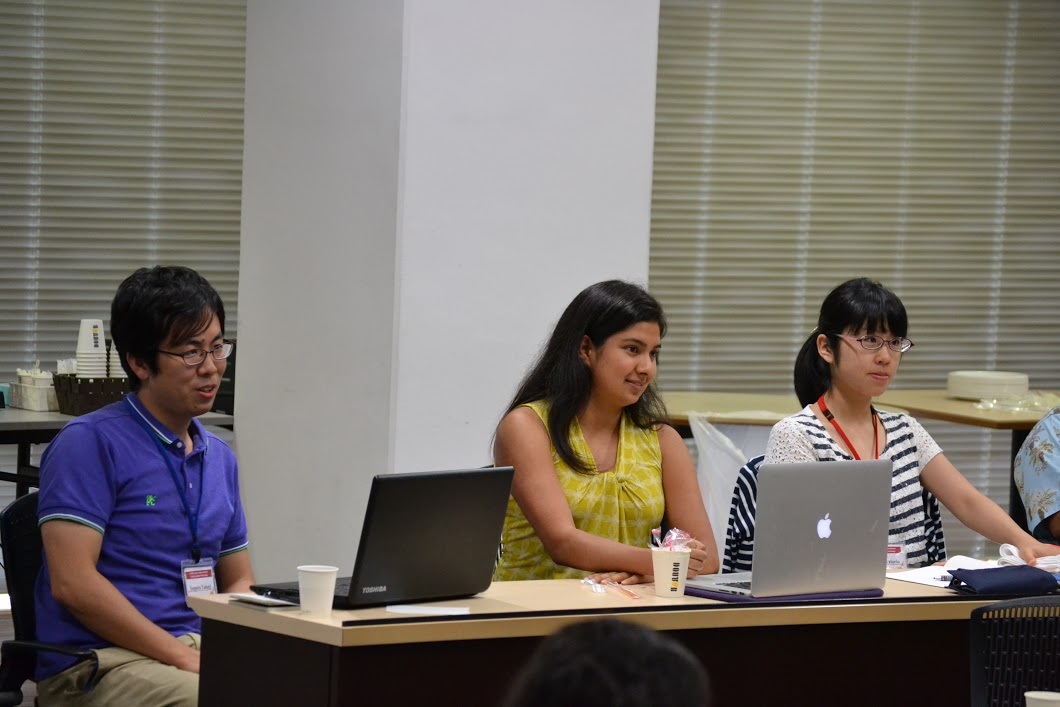
\includegraphics[width=0.4\textwidth]{presentations_audience.JPG}}\\
    
    \subfigure{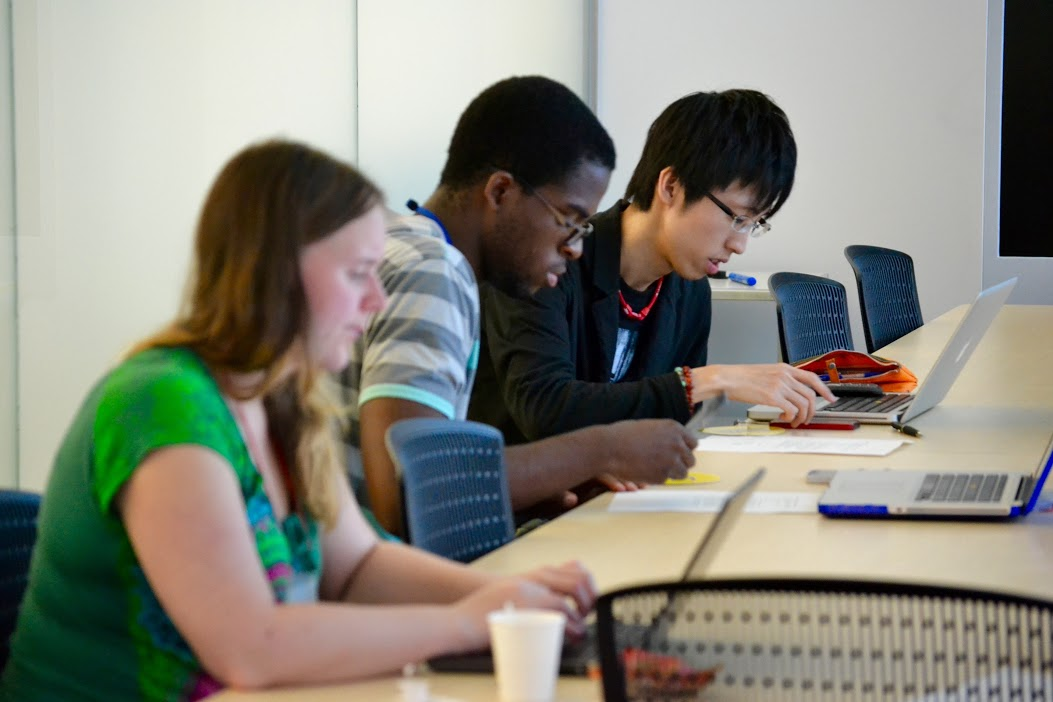
\includegraphics[width=0.4\textwidth]{students_on_computers.jpg}}
    \subfigure{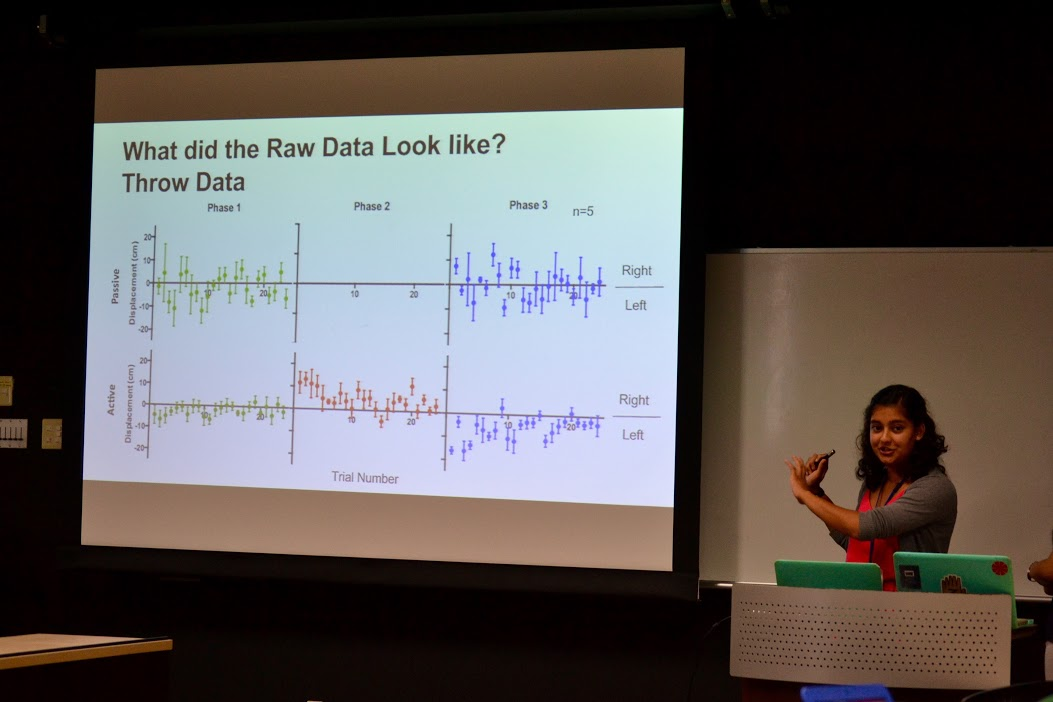
\includegraphics[width=0.4\textwidth]{student_presenting.jpg}}  
\end{figure}
\end{frame}

\begin{frame}
\frametitle{Als Mediziner*in sollten Sie wissenschaftlich arbeiten können - Aber wie? Und warum? Und was heißt das?}

\begin{figure}
    \centering
    \subfigure{\includegraphics[width=0.4\textwidth]{collaborative_experiment.png}} 
    \subfigure{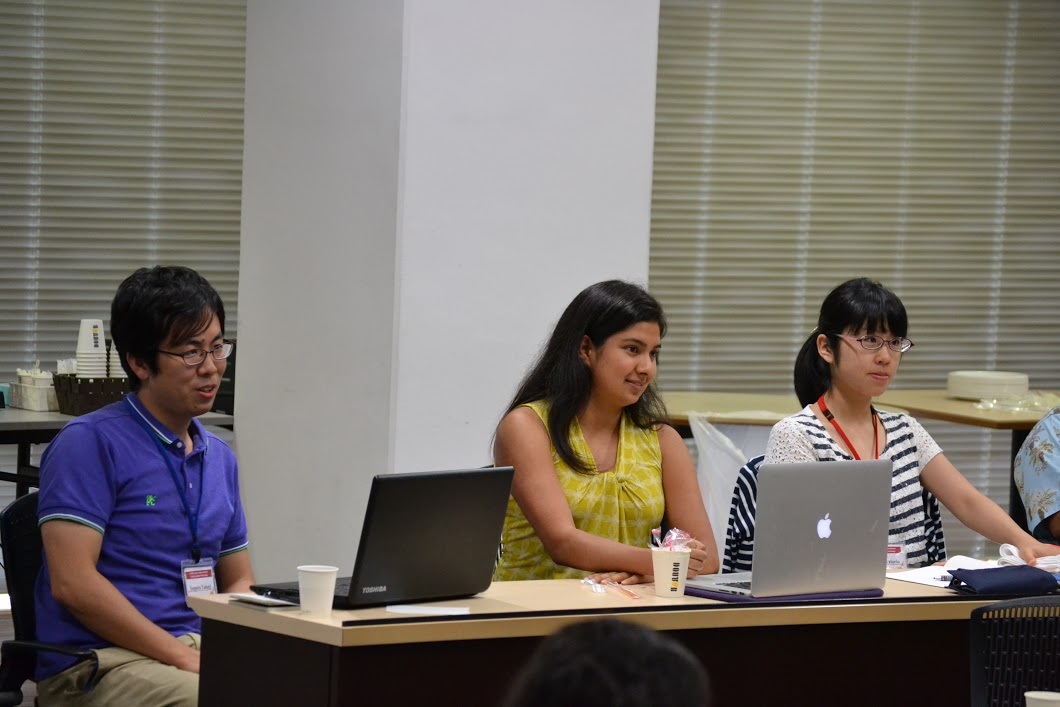
\includegraphics[width=0.4\textwidth]{presentations_audience.JPG}}\\
    
    \subfigure{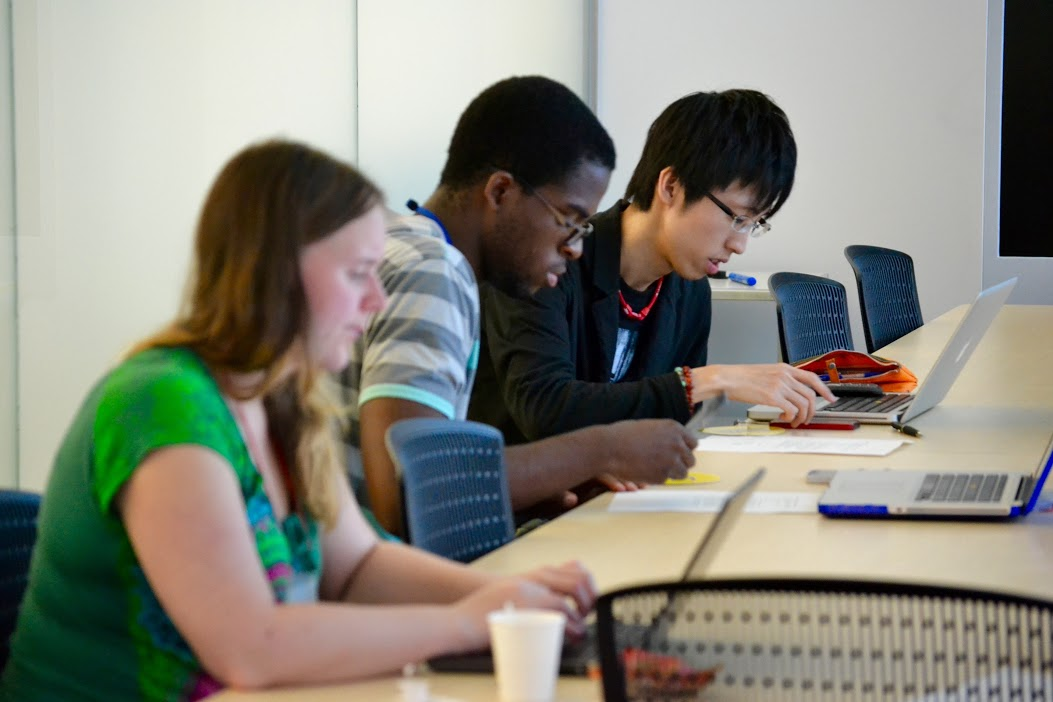
\includegraphics[width=0.4\textwidth]{students_on_computers.jpg}}
    \subfigure{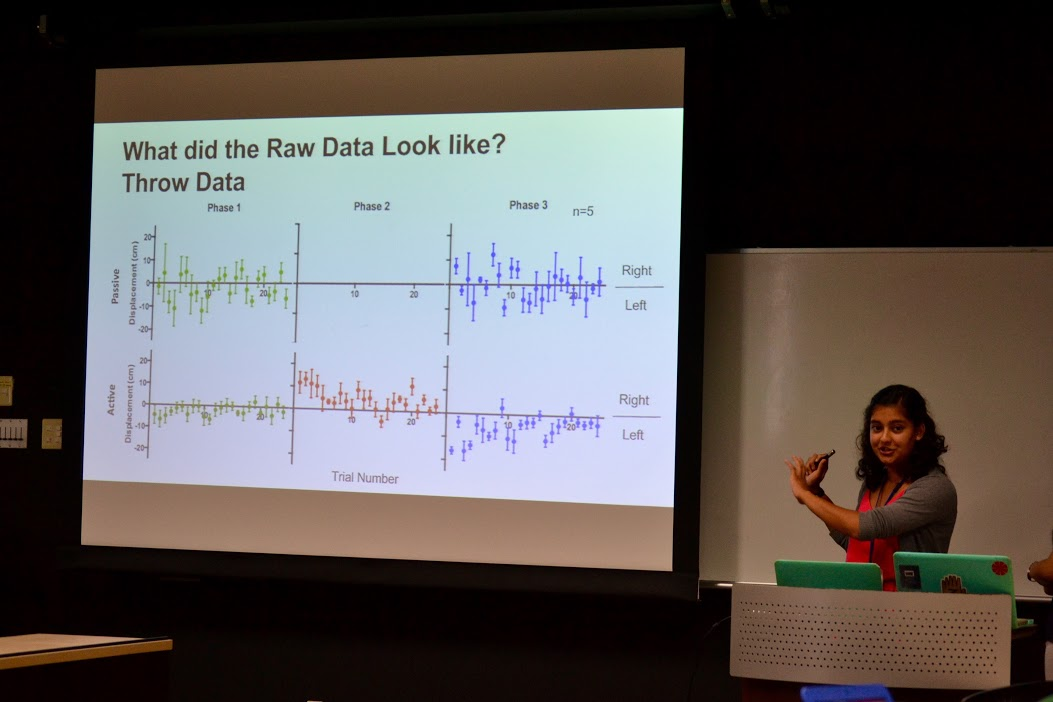
\includegraphics[width=0.4\textwidth]{student_presenting.jpg}}  
\end{figure}
\end{frame}



%% TLIA
%\begin{frame}
%\frametitle{In dieser Vorlesung geht es um\dots}
%



%\end{frame}


%% Learning Objectives
 
\begin{frame}

\frametitle{Nach dieser Vorlesung sollten Sie:}



\begin{block}{Wissen:}
\begin{itemize}
%%%%%
\item
Wissen, was Ihnen im Modul M14 bevorsteht und wie Sie benotet werden

\item
Wichtige historische Entwicklungen benennen
\item 
Grundbegriffe der Erkenntnistheorie benennen und erklären
\item 
Die Grundlagen des kritischen Rationalismus benennen und erklären
\item 
Häufige Denkfehler benennen und anhand von Beispielen erläutern
\end{itemize}

\end{block}

 

\begin{block}{Können:}
\begin{itemize}
\item
Den historischen und gesellschaftlichen Kontext wissenschaftlicher Forschung erkennen
\item 
Wissenschaftliche Forschung kritisch reflektieren
\item 
Häufige Denkfehler erkennen und vermeiden
\end{itemize}
\end{block}

\end{frame}


\begin{frame}

\frametitle{Nach dieser Vorlesung sollten Sie:}

\begin{block}{Fühlen:}

\begin{itemize}
\item
Ihre Rolle als medizinische*r Gelehrte*r reflektieren
\item 
Eine kritische wissenschaftliche Haltung entwickeln
\item 
Sich auf M14 freuen $\heart$
\end{itemize}

\end{block}


\end{frame}


%% Main Body

\section{Willkommen in M14}

%% Warum sind Sie hier?

\begin{frame}{Warum sind Sie hier?}

\begin{itemize}
    \item 
Wollen Sie wissenschaftlich arbeiten?
\item 
Was bedeutet überhaupt  ``wissenschaftliches Arbeiten'' für Sie? 
\item 
Wie wird das in Ihrem späteren Berufsleben relevant sein? 
    
\end{itemize}
    
\end{frame}

%% CanMEDS rollen
\begin{frame}{Warum sind Sie hier?}


\end{frame}


%% Warum bin ich hier?

%% Was erwartet uns?

\section{Wissenschaftsgeschichte}

%% Woher wissen wir die Dinge, die wir wissen?

%% Wissenschaftsgeschichte


\section{Wissenschaftslehre und Erkenntnistheorie}

%% wissenschaftslehre, kritischer Rationalismus

%% Fallen


%% Review


\begin{frame}

\frametitle{Jetzt* sollten Sie:}



\begin{block}{Wissen:}
\begin{itemize}
%%%%%
\item
Wissen, was Ihnen im Modul M14 bevorsteht und wie Sie benotet werden

\item
Wichtige historische Entwicklungen benennen
\item 
Grundbegriffe der Erkenntnistheorie benennen und erklären
\item 
Die Grundlagen des kritischen Rationalismus benennen und erklären
\item 
Häufige Denkfehler benennen und anhand von Beispielen erläutern
\end{itemize}

\end{block}

 

\begin{block}{Können:}
\begin{itemize}
\item
Den historischen und gesellschaftlichen Kontext wissenschaftlicher Forschung erkennen
\item 
Wissenschaftliche Forschung kritisch reflektieren
\item 
Häufige Denkfehler erkennen und vermeiden
\end{itemize}
\end{block}

\end{frame}


\begin{frame}

\frametitle{Jetzt* sollten Sie:}

\begin{block}{Fühlen:}

\begin{itemize}
\item
Ihre Rolle als medizinische*r Gelehrte*r reflektieren
\item 
Eine kritische wissenschaftliche Haltung entwickeln
\item 
Sich auf M14 freuen $\heart$
\end{itemize}

\end{block}


\end{frame}


%% Feedbackhinweisblock

\begin{frame}
\frametitle{Danke für Ihr Feedback!}
\begin{center}

\includegraphics[width=0.6\textwidth]{feedback_QR.png}
\end{center}

\end{frame}





%% Bildnachweis
\begin{frame}
\frametitle{Bildnachweis}

\vfill

\begin{tiny}
 
\begin{itemize}

%% all lectures
\item
Logo der MSB. MSB Medical School Berlin, Public Domain, via Wikimedia Commons
\item 
Studierende beim gemeinsamen Experimentieren, bei der Arbeit an ihren Computern und beim Präsentieren von Daten. Yuuki Guzman und Agoston Tyll, Okinawa Institute of Science and Technology, 2015 und 2016. 
\end{itemize}
\end{tiny}
\end{frame}


\end{document}
